\documentclass[11pt, letterpaper, includehead]{article}

%%%%%%%%%%%%%%%%%%%%% Pre-document %%%%%%%%%%%%%%%%%%%%%
\usepackage{fancyhdr}  % Allow for headers
\usepackage{graphicx}  % Allow for figures 
\usepackage{float}     % Allow for figure inserted in specified location

\setlength{\parindent}{0pt} % Remove auto paragraph indents

% Get rid of those big ass margins
\usepackage[margin=1in]{geometry}

% Table cell formatting
\setlength{\arrayrulewidth}{0.25mm}
\setlength{\tabcolsep}{11pt}
\renewcommand{\arraystretch}{1.2}

\begin{document}

$$\sum F = F_{1} + F_{2}$$

$$|F_1| = mg$$
$$|F_1| = 35g(9.80m/s^2)$$
$$|F_1| = 343N$$

$$|F_2| = mg$$
$$|F_2| = 55g(9.80m/s^2)$$
$$|F_2| = 343N$$

$$F_{1x} = |F_1|\cos\theta$$
$$F_{1x} = 343N(\cos60^{\circ})$$
$$F_{1x} = 171.5N$$

$$F_{1y} = |F_1|\sin\theta$$
$$F_{1y} = 343N(\sin^{\circ})$$
$$F_{1y} = 171.5N$$

$$F_{2x} = |F_2|\cos\theta$$

$$F_{2y} = |F_2|\sin\theta$$


%%%%%%%%%%%%%%%%%%%%% Title Page %%%%%%%%%%%%%%%%%%%%%
\begin{titlepage}
  \begin{center}
    \Huge{\textbf{Lab 3}}\\
    \Huge{Vectors}
    \vfill
    \begin{figure}[H] % H makes the figure insert at the position in the document
      \centering 
      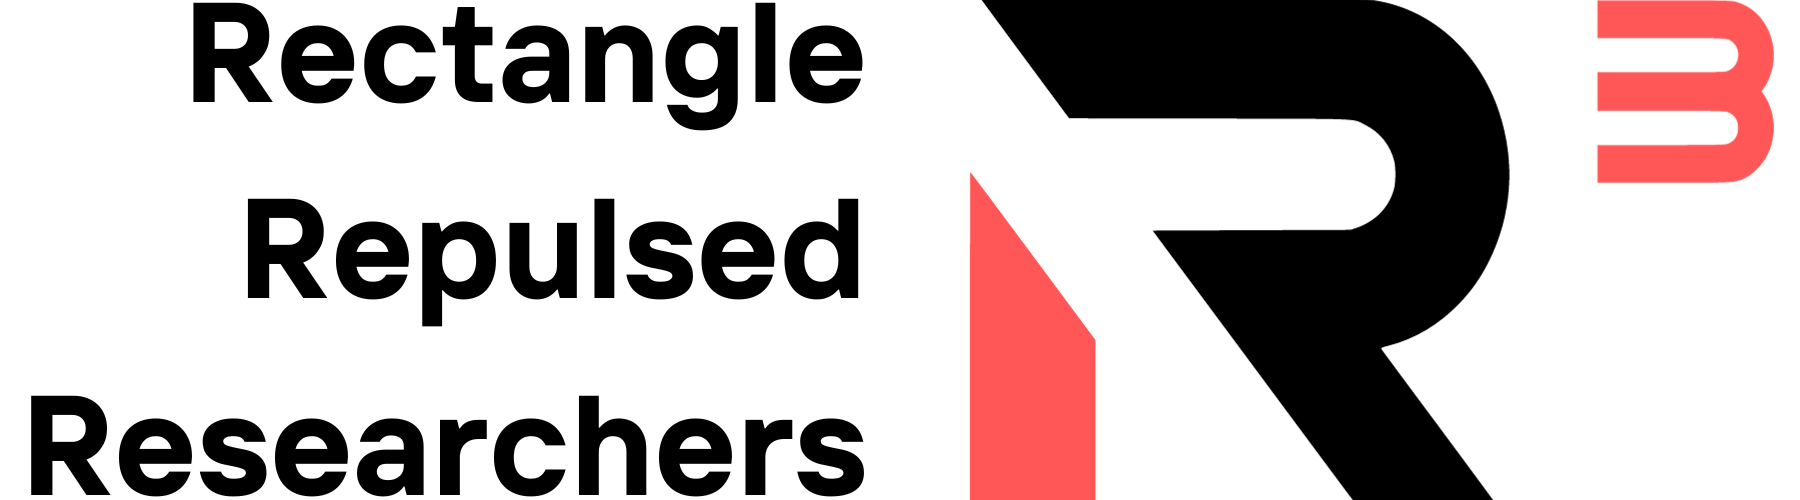
\includegraphics[width=6cm]{../logo.png}
    \end{figure}
    \large{\textbf{Rectangle Repulsed Researchers}}\\
    \large{Julian Barossi, Liam Gilligan, Stephanie L'Heureux}\\
    \vspace{0.5cm}
    \normalsize
    \today
  \end{center}
\end{titlepage}

%%%%%%%%%%%%%%%%%%%%% TABLE OF CONTENTS %%%%%%%%%%%%%%%%%%%%%
\tableofcontents
\pagebreak % Move to next page

% Add a nice fancy header
\pagestyle{fancy}
\fancyhead{}
\fancyhead[C]{\textbf{Lab 3:} Vectors}

\pagebreak 

%%%%%%%%%%%%%%%%%%%%% ADDING TWO VECTORS %%%%%%%%%%%%%%%%%%%%%
\section{Adding Two Vectors} % 1

%%%%%%%%%%%%%%%%%%%%% GIVEN VECTORS %%%%%%%%%%%%%%%%%%%%%
\subsection{Given vectors} % 1.1

\subsubsection{Find components} % 1.1.1

\subsubsection{Two forces to balance the net force} % 1.1.2

\subsubsection{Was the prediction correct} % 1.1.3

\subsubsection{Single forces to balance the net force} % 1.1.4

\subsubsection{Was the prediction correct} % 1.1.5

%%%%%%%%%%%%%%%%%%% CHOSEN VECTORS %%%%%%%%%%%%%%%%%%%%%
\subsection{Chosen vectors} % 1.2

\subsubsection{Find components} % 1.2.1

\subsubsection{Two forces to balance the net force} % 1.2.2

\subsubsection{Was the prediction correct} % 1.2.3

\subsubsection{Single forces to balance the net force} % 1.2.4

\subsubsection{Was the prediction correct} % 1.2.5

%%%%%%%%%%%%%%%%%%% ADDING THREE VECTORS %%%%%%%%%%%%%%%%%%%%%
\section{Adding three vectors} % 2

%%%%%%%%%%%%%%%%%%%%% GIVEN VECTORS %%%%%%%%%%%%%%%%%%%%%
\subsection{Given vectors} % 2.1

\subsubsection{Find components} % 2.1.1

\subsubsection{Single forces to balance the net force} % 2.1.2

\subsubsection{Was the prediction correct} % 2.1.3

%%%%%%%%%%%%%%%%%%%%% CHOSEN VECTORS %%%%%%%%%%%%%%%%%%%%%
\subsection{Given vectors} % 2.2

\subsubsection{Find components} % 2.2.1

\subsubsection{Single forces to balance the net force} % 2.2.2

\subsubsection{Was the prediction correct} % 2.2.3

%%%%%%%%%%%%%%%%%%% BURIED TREASURE %%%%%%%%%%%%%%%%%%%%%
\section{Hunt for Buried Treasure} % 3
\subsection{Game A} % 3.1
\subsection{Game B} % 3.2
\subsection{Game C} % 3.3

\end{document}